\subsection{Linux development process}

\begin{frame}[fragile]
  \frametitle{What's new in each Linux release? (1)}
  The official list of changes for each Linux release is just a
  huge list of individual patches!
\Tiny
    \begin{verbatim}
commit aa6e52a35d388e730f4df0ec2ec48294590cc459
Author: Thomas Petazzoni <thomas.petazzoni@bootlin.com>
Date:   Wed Jul 13 11:29:17 2011 +0200

    at91: at91-ohci: support overcurrent notification

    Several USB power switches (AIC1526 or MIC2026) have a digital output
    that is used to notify that an overcurrent situation is taking
    place. This digital outputs are typically connected to GPIO inputs of
    the processor and can be used to be notified of these overcurrent
    situations.

    Therefore, we add a new overcurrent_pin[] array in the at91_usbh_data
    structure so that boards can tell the AT91 OHCI driver which pins are
    used for the overcurrent notification, and an overcurrent_supported
    boolean to tell the driver whether overcurrent is supported or not.

    The code has been largely borrowed from ohci-da8xx.c and
    ohci-s3c2410.c.

    Signed-off-by: Thomas Petazzoni <thomas.petazzoni@bootlin.com>
    Signed-off-by: Nicolas Ferre <nicolas.ferre@atmel.com>
\end{verbatim}
\normalsize
  Very difficult to find out the key changes and to get the
  global picture out of individual changes.
\end{frame}

\begin{frame}
  \frametitle{What's new in each Linux release? (2)}
  Fortunately, there are some useful resources available
  \begin{itemize}
    \item \url{https://kernelnewbies.org/LinuxChanges}\\
	In depth coverage of the new features in each kernel release
    \item \url{https://lwn.net/Kernel}\\
	Coverage of the features accepted in each merge window
  \end{itemize}
  \begin{center}
    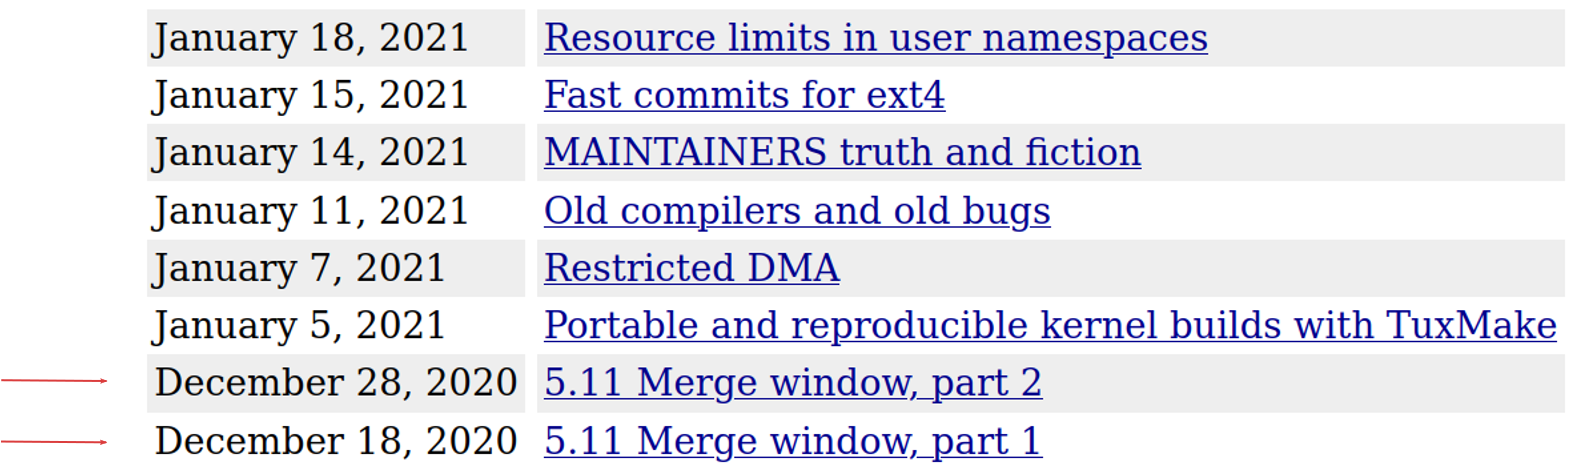
\includegraphics[width=0.8\textwidth]{common/lwn-kernel-articles.pdf}
  \end{center}
\end{frame}
